\section{Bounds on the susceptibility score}
\label{app:susc}
In Theorem \ref{thm:linlinf}, we give non-asymptotic bounds on the robust and standard error of a linear classifier trained with adversarial logistic regression. Moreover, we use the robust error decomposition in susceptibility and standard error to gain intuition about how adversarial training may hurt robust generalization. In this section, we complete the result of Theorem \ref{thm:linlinf} by also deriving non-asymptotic bounds on the susceptibility score of the max $\ell_2$-margin classifier.

Using the results in Appendix \ref{sec:app_theorylinear}, we can prove following Corollary \ref{cor:robustness}, which gives non asymptotic bounds on the susceptibility score.
\begin{corollary}
\label{cor:robustness}
  Assume $d-1>n$. For the $\epstest$-susceptibility on test samples from $\prob_{\sigsep}$ with $2 \epstest < \sigsep$ and perturbation sets in Equation~\eqref{eq:linfmaxpert} and~\eqref{eq:l1maxpert} the following holds:

For $\epstrain < \frac{\sigsep}{2} - \maxmargin$, with probability at least $1-2\E^{-\frac{\tconst^2 (d-1)}{2}}$ for any $0<\tconst<1$, over the draw of a dataset $\data$ with $n$ samples from $\prob_{\sigsep}$, the $\epstest$-susceptibility is upper and lower bounded by
  \begin{equation}
  \begin{split}
       &\suscept{\thetaA} \leq \Phi \left(\frac{(\sigsep-2 \epstrain) (\epstest - \frac{\sigsep}{2})}{2 \maxmargin \sigma}\right) - \Phi \left( \frac{(\sigsep-2 \epstrain)( -\epstest - \frac{\sigsep}{2})}{2 \minmargin\sigma} \right)\\ 
       &\suscept{\thetaA} \geq   \Phi \left(\frac{(\sigsep-2 \epstrain) (\epstest - \frac{\sigsep}{2})}{2 \minmargin\sigma}\right) - \Phi \left( \frac{(\sigsep-2 \epstrain)( -\epstest - \frac{\sigsep}{2})}{2 \maxmargin \sigma} \right)
        \end{split}
  \end{equation}
\end{corollary}

We give the proof in Subsection \ref{sec:proof_robust_cor}. Observe that the bounds on the susceptibility score in Corollary \ref{cor:robustness} consist of two terms each, where the second term decreases with $\epstrain$, but the first term increases. We recognise following two regimes: the max $\ell_2$-margin classifier is close to the ground truth $e_1$ or not. Clearly, the ground truth classifier has zero susceptibility and hence classifiers close to the ground truth also have low susceptibility. On the other hand, if the max $l_2$-margin classifier is not close to the ground truth, then putting less weight on the first coordinate increases invariance to the perturbations along the first direction. Recall that by Lemma \ref{lem:maxmargin}, increasing $\epstrain$, decreases the weight on the first coordinate of the max $\ell_2$-margin classifier. Furthermore, in the low sample size regime, we are likely not close to the ground truth. Therefore, the regime where the susceptibility decreases with increasing $\epstrain$ dominates in the low sample size regime.

To confirm the result of Corollary \ref{cor:robustness}, we plot the mean and standard deviation of the susceptibility score of $5$ independent experiments. The results are depicted in Figure \ref{fig:logreg_robust}. We see that for low standard error, when the classifier is reasonably close to the optimal classifier, the susceptibility increases slightly with increasing adversarial budget. However, increasing the adversarial training budget, $\epstrain$, further, causes the susceptibility score to drop greatly. Hence, we can recognize both regimes and validate that, indeed, the second regime dominates in the low sample size setting.

%%\paragraph{Intuition} We note the following two regimes.
%%\begin{enumerate}
%%\item The robust max $l_2$-margin classifier, $\thetaA$, is close to the ground truth $e_1$. Recall that the classifier induced by $e_1$ achieves zero robust error, and hence also achieves zero susceptibility. In consequence, classifiers close to $e_1$ have low susceptibility scores as well. Because, by Lemma \ref{lem:maxmargin}, increasing $\epstrain$ tilts the resulting classifier away from $e_1$, we expect the susceptibility to increase with increasing $\epstrain$ in this regime. 

%%\item The robust max $l_2$-margin classifier, $\thetaA$, is not close to the ground truth $e_1$. We first note that in the low sample size regime, $\thetaA$ is likely not that close to $e_1$. In this case, the more weight on the first coordinate of $\thetaA$ the more influence a perturbation along the first coordinate has. The more influence the perturbation has, the likelier it can change the prediction label of the sample, which means the more susceptible the classifier. By Lemma \ref{lem:maxmargin}, the larger $\epstrain$, the lower the weight on the first coordinate of  $\thetaA$ and hence the less susceptible the classifier.
%%\end{enumerate}

%%Putting regimes $1$ and $2$ together, we find that if $\sigsep$ is large, we expect a U-form for the susceptibility score over a large range of $\epstrain$. First, the classifier is close to the ground truth and therefore has a low susceptibility score. Then, by increasing $\epstrain$ we tilt the classifier away from $e_1$, which at first increases the susceptibility. Thereafter, when the classifier is not close to $e_1$, increasing $\epstrain$ reduces the weight on the first coordinate of $\thetaA$, which decreases the susceptibility of $\thetaA$ again. Lastly, increasing $\epstrain$ to the limit causes the first coordinate of  $\thetaA$ to approximate $0$, which results in a fully non-susceptible classifier.

%% However, since we are particularly interested in the low sample size regime with a reasonable $\sigsep$, we find that regime $2$ characterizes the setting of this paper. 
 

 
 \begin{figure*}[!b]
  \centering
\begin{subfigure}[b]{0.4\textwidth}
 \centering
  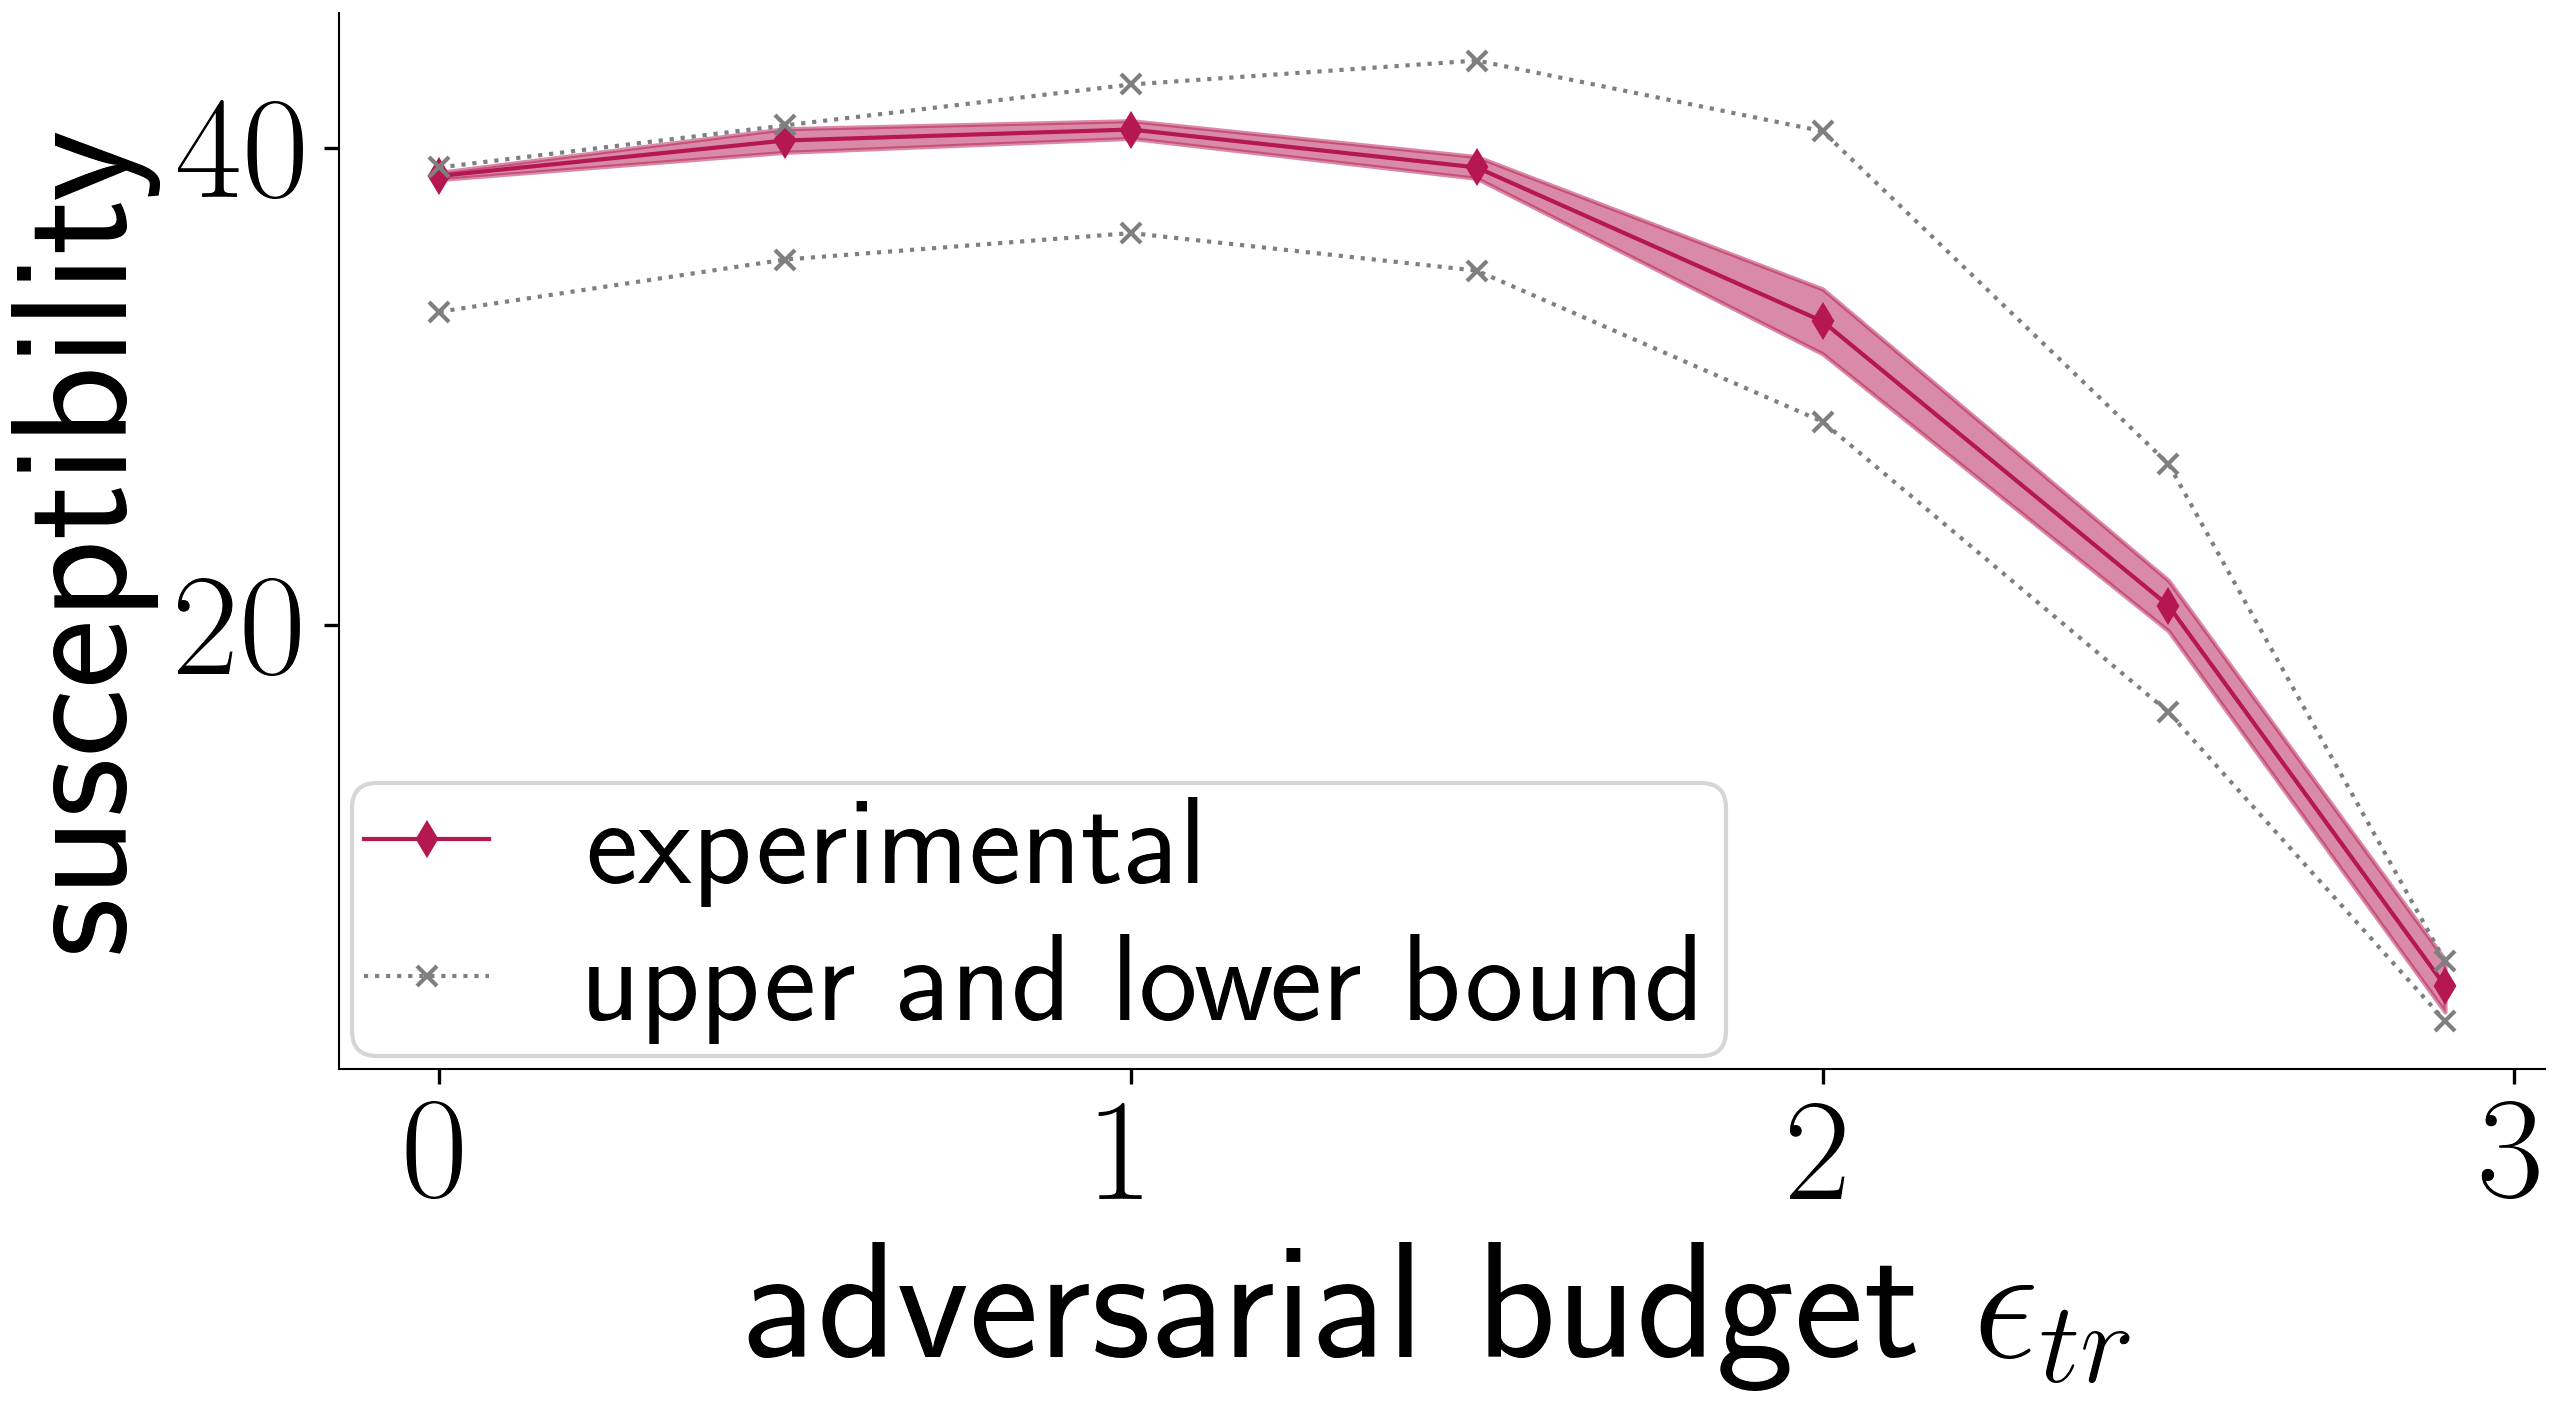
\includegraphics[width=0.99\linewidth]{plotsAistats/app_susceptibilty.png}
  \caption{Susceptibility score decreases with $\epstrain$}
  \label{fig:app_robustness}
\end{subfigure}
\begin{subfigure}[b]{0.4\textwidth}
 \centering
  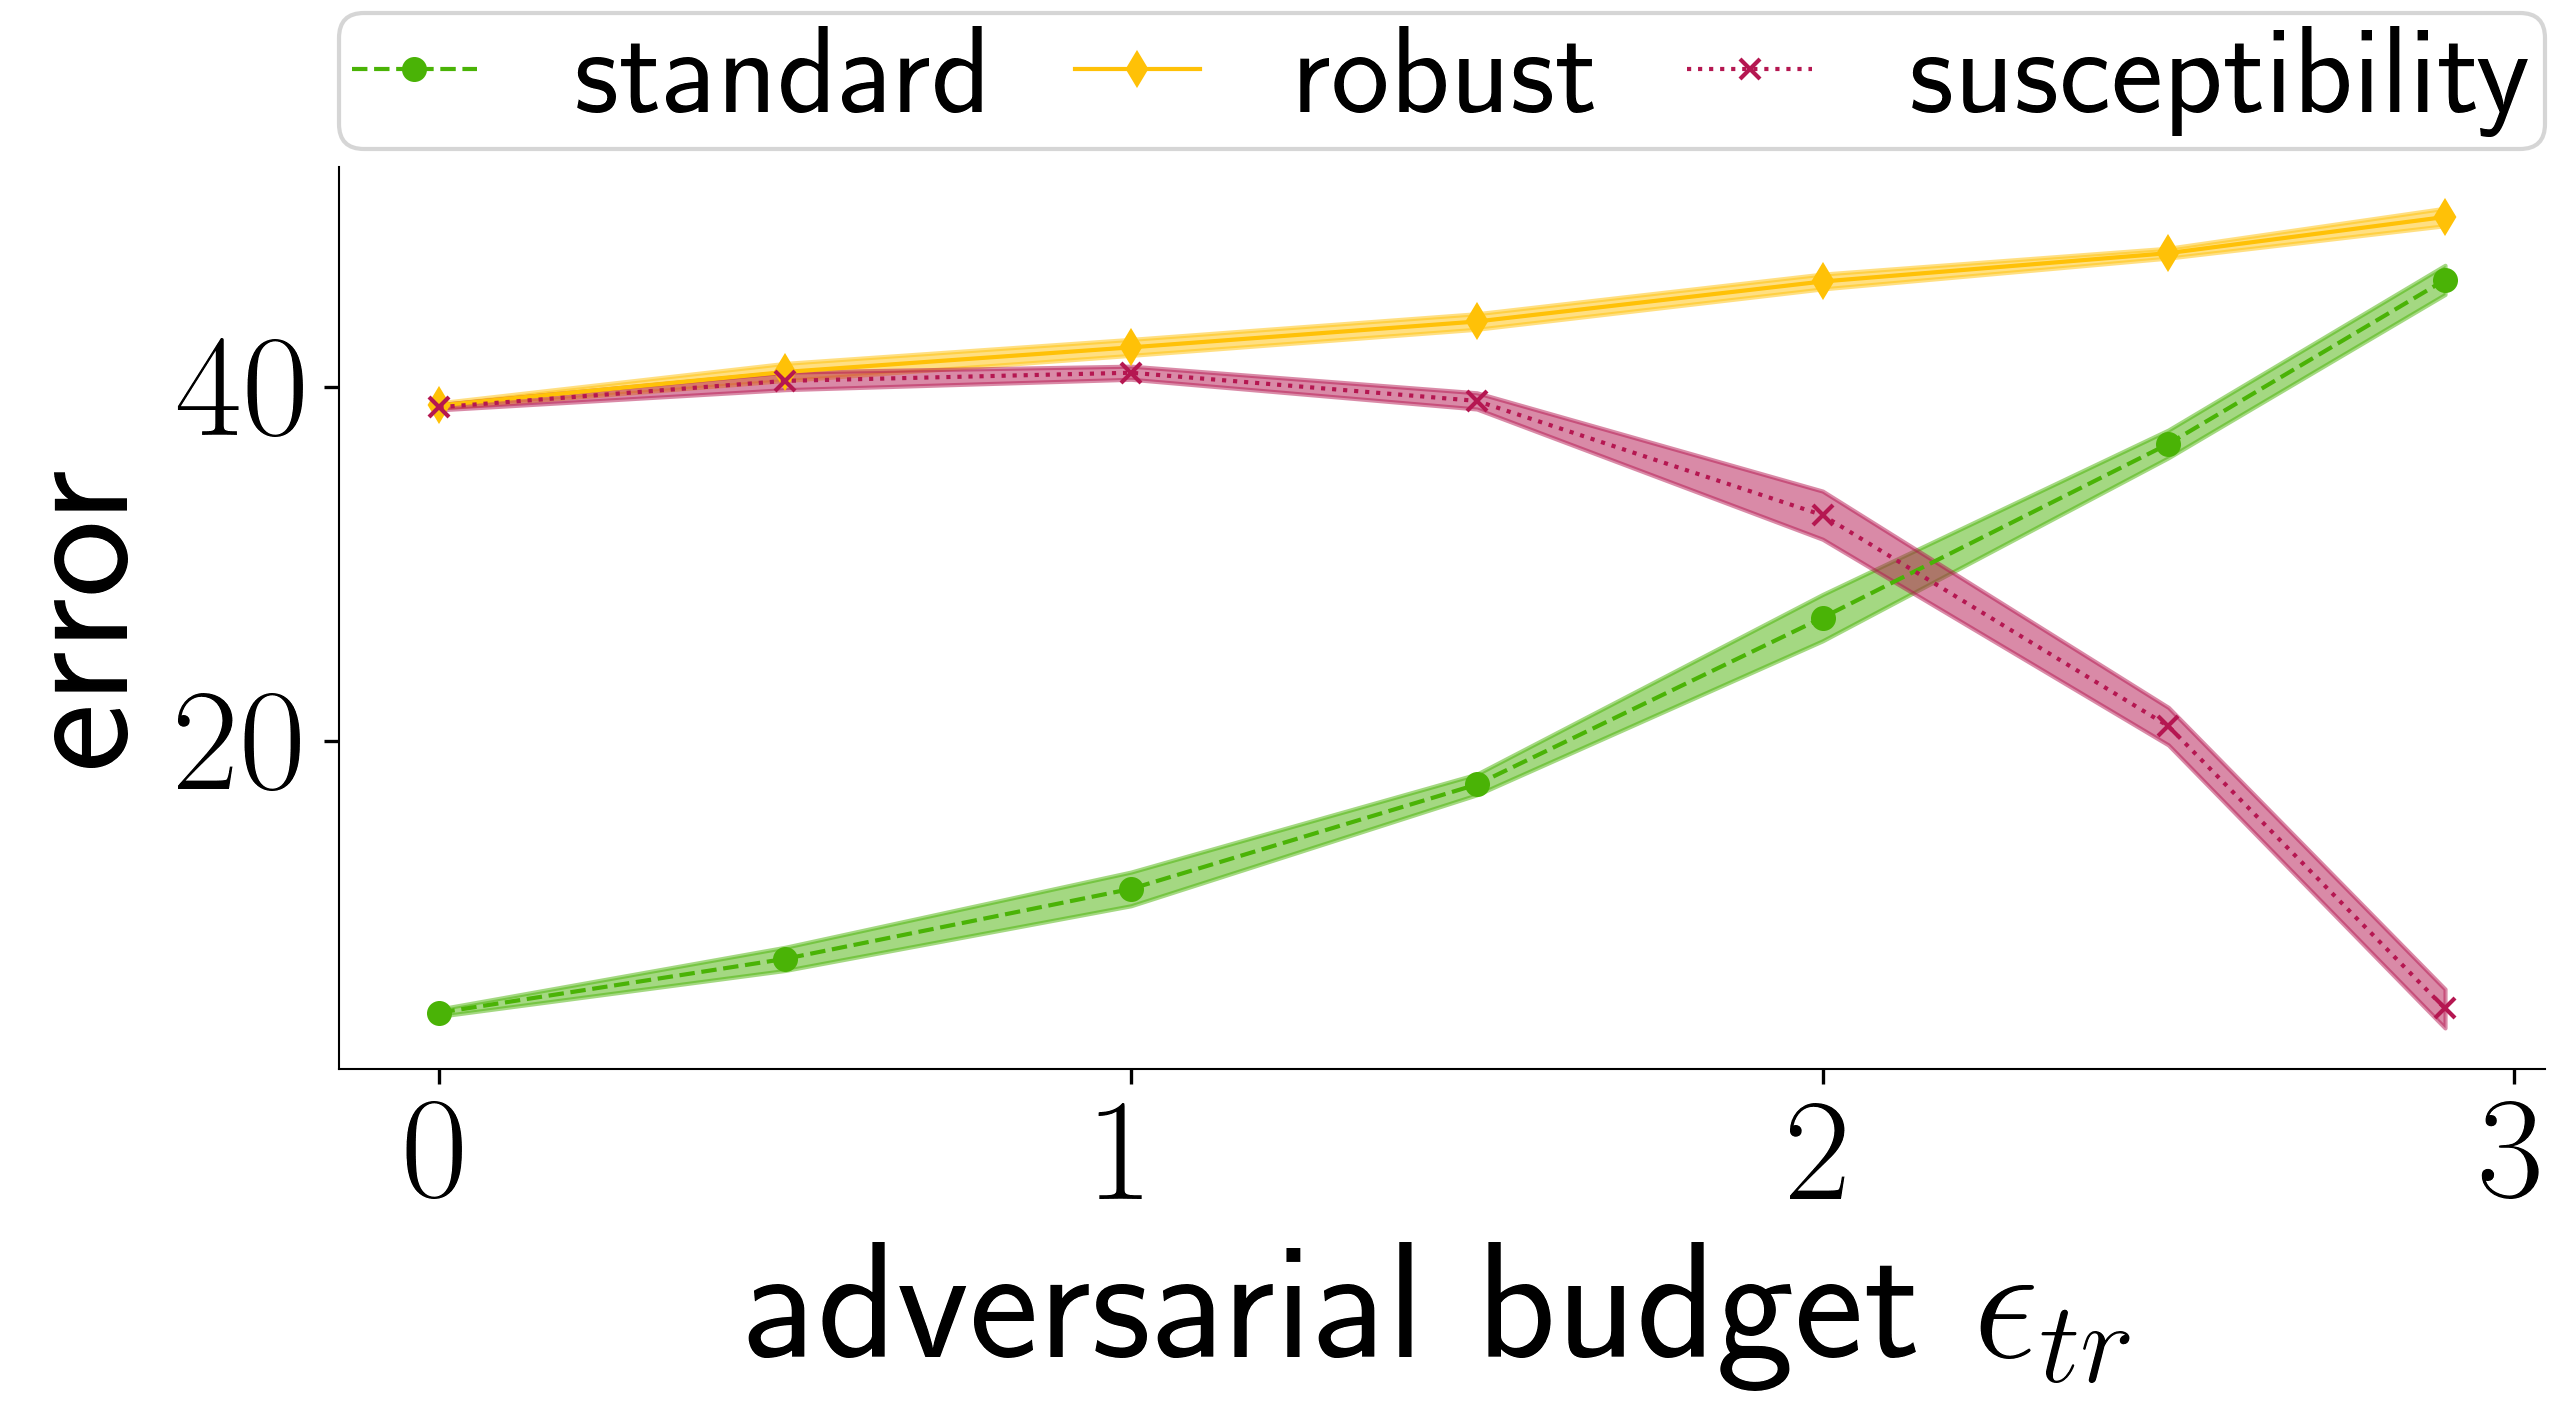
\includegraphics[width=0.99\linewidth]{plotsAistats/logreg_trade_off_plot.png}
  \caption{Robust error decomposition}
  \label{fig:app_tradeoff_logreg}
\end{subfigure}
\caption{We set $\sigsep = 6$, $\dims = 1000$, $\numsamp = 50$ and $\epstest = 2.5$. (a) We plot the average susceptibility score and the standard deviation over 5 independent experiments. Note how the bounds closely predict the susceptibility score. (b) For comparison, we also plot the robust error decomposition in susceptibility and standard error. Even though the susceptibility decreases, the robust error increases with increasing adversarial budget $\epstrain$.}
  \vspace{-0.2in}
\label{fig:logreg_robust}
\end{figure*}

\subsection{Proof of Corollary \ref{cor:robustness}}
\label{sec:proof_robust_cor}
We proof the statement by bounding the robustness of a linear classifier. Recall that the robustness of a classifier is the probability that a classifier does not change its prediction under an adversarial attack. The susceptibility score is then given by 
\begin{equation}
\label{eq:rob_sus}
\suscept{\thetaA} = 1 - \robness{\thetaA}.
\end{equation}

The proof idea is as follows: since the perturbations are along the first basis direction, $e_1$, we compute the distance from the robust $l_2$-max margin $\thetaA$ to a point $(X,Y) \sim \prob$. Then, we note that the robustness of $\thetaA$ is given by the probability that the distance along $e_1$, from $X$ to the decision plane induced by $\thetaA$ is greater then $\epstest$. Lastly, we use the non-asymptotic bounds of Lemma \ref{lem:boundsmaxmargin}.

Recall, by Lemma \ref{lem:maxmargin}, the max $l_2$-margin classifier is of the form of
\begin{equation}
\label{eq:robustmaxmarg}
\thetaA = \frac{1}{\sqrt{(\sigsep-2 \epstrain)^2 + 4 \marginnonsig^{2}}}\left[\sigsep-2\epstrain,  2 \marginnonsig \thetatilde \right].
\end{equation}
Let $(X, Y) \sim \prob$. The distance along $e_1$ from $X$ to the decision plane induced by $\thetaA$, $\decplanegen{\thetaA }$, is given by
\begin{equation*}
d_{e_1}(X, \decplanegen{\thetaA}) = \left| \indof{X}{1}+ \frac{1}{ \indof{\thetaA}{0}} \sum_{i=2}^{ \dims }  \indof{\thetaA}{i} \indof{X}{i} \right|. 
\end{equation*}
Substituting the expression of $\thetaA$ in Equation \ref{eq:robustmaxmarg} yields
\begin{equation*}
d_{e_1}(X, \decplanegen{\thetaA}) = \left| \indof{X}{1} + 2 \marginnonsig \frac{1}{(\sigsep-\epstrain)} \sum_{i=2}^{\dims}  \indof{\thetatilde}{i}   \indof{X}{i} \right|. 
\end{equation*}
Let $N$ be a standard normal distributed random variable. By definition $\| \thetatilde\|_2^2 = 1$ and using that a sum of Gaussian random variables is again a Gaussian random variable, we can write 
\begin{equation*}
d_{e_1}(X,\decplanegen{\thetaA}) = \left| \indof{X}{1} + 2 \marginnonsig \frac{\sigma}{(\sigsep-\epstrain)} N \right|. 
\end{equation*}
The robustness of $\thetaA$ is given by the probability that $d_{e_1}(X,\decplanegen{\thetaA}) > \epstest$. Hence, using that $X_1 = \pm \frac{\sigsep}{2}$ with probability $\frac{1}{2}$, we get
\begin{equation}
\label{eq:robustness_form}
\robness{\thetaA} = P\left[ \frac{\sigsep}{2} + 2 \marginnonsig \frac{\sigma}{(\sigsep-2\epstrain)}  N > \epstest \right] + P \left[ \frac{\sigsep}{2} + 2 \marginnonsig \frac{\sigma}{(\sigsep-\epstrain)}  N < -\epstest \right].
\end{equation}
We can rewrite Equation \ref{eq:robustness_form} in the form
\begin{equation*}
\robness{\thetaA}  = P \left[ N > \frac{(\sigsep-2\epstrain) (\epstest - \frac{\sigsep}{2})}{2 \marginnonsig\sigma} \right] + P \left[  N <  \frac{(\sigsep-2\epstrain)( -\epstest -\frac{ \sigsep}{2})}{2 \marginnonsig\sigma} \right].
\end{equation*}
Recall, that $N$ is a standard normal distributed random variable and denote by $\Phi$ the cumulative standard normal density. By definition of the cumulative denisity function, we find that
\begin{equation*}
\robness{\thetaA} = 1 - \Phi \left(\frac{(\sigsep-2\epstrain) (\epstest - \frac{\sigsep}{2})}{2 \marginnonsig\sigma}\right) + \Phi \left( \frac{(\sigsep-2 \epstrain)( -\epstest - \frac{\sigsep}{2})}{2 \marginnonsig\sigma} \right).
\end{equation*}
Substituting the bounds on $\marginnonsig$ of Lemma \ref{lem:boundsmaxmargin} gives us the non-asymptotic bounds on the robustness score and by Equation \ref{eq:rob_sus} also on the susceptibility score.  


\section{Experimental details on the linear model}

\label{sec:logregapp}
In this section, we provide detailed experimental details to Figures \ref{fig:main_theorem} and \ref{fig:lineartradeoff}.

We implement adversarial logistic regression using stochastic gradient descent with a learning rate of $0.01$. Note that logistic regression converges logarithmically to the robust max $l_2$-margin solution. As a consequence of the slow convergence, we train for up to $10^7$ epochs. Both during training and test time we solve $\max_{x_i' \in \pertset{x_i}{\epstrain}} \loss(f_\theta(x_i') y_i)$ exactly. Hence, we exactly measure the robust error. %%Let $(x,y) \sim \lgdistribution$, then the inner maximization is given by
%\begin{equation*}
%\argmax_{x' \in \pertset{x}{\epstrain}} \loss(f_\theta(x') y) = x - y \epstrain \text{sign}\left(\theta_{j^{\ast}(\theta)} \right)e_{j^{\ast}(\theta)}.
%\end{equation*}
%At test time we use exact evaluation of the inner maximization and hence work with so-called robustness certificates for robust evaluation \cite{Wong18}. 
Unless specified otherwise, we set $\mixvar= 1$,  $\sigsep = 12$ and $\epstest = 4$. 

\paragraph{Experimental details on Figure \ref{fig:main_theorem}} (a) We draw $5$ datasets with $\numsamp= 50$ samples and input dimension $\dims=1000$ from the distribution $\prob$. We then run adversarial logistic regression on all $5$ datasets with adversarial training budgets, $\epstrain = 1$ to $5$. To compute the resulting robust error gap of all the obtained classifiers, we use a test set of size $10^{6}$. Lastly, we compute the lower bound given in part 2. of Theorem \ref{thm:linlinf}. (b) We draw $5$ datasets with different sizes $\numsamp$ between $50$ and $10^4$. We take an input dimension of $d = 10^4$ and plot the mean and standard deviation of the robust error after adversarial and standard logistic regression over the $5$ samples.(c) We again draw $5$ datasets for each $d/n$ constellation and compute the robust error gap for each dataset.

\paragraph{Experimental details on Figure \ref{fig:lineartradeoff}} For both (a) and (b) we set $\dims = 1000$, $\epstest = 4$, and vary the adversarial training budget ($\epstrain$) from $1$ to $5$. For every constellation of $\numsamp$ and $\epstrain$, we draw $10$ datasets and show the average and standard deviation of the resulting robust errors. In (b), we set $\numsamp = 50$.

%\begin{figure}[!ht]
%\centering
%  \includegraphics[width=0.6\linewidth]{plotsAistats/logreg_numobs_full.png}
%  \caption{We plot the robust accuracy after standard and adversarial training with increasing number of samples (we run on $20$ different datasets per dataset size  and show the mean). For a large number of samples adversarial training has an as high robust accuracy as standard training, which are both near perfect.}
%\label{fig:logreg_numobs_full}
%\end{figure}







